\documentclass[letterpaper, titlepage, 10pt]{article}

\usepackage[margin=4cm]{geometry}
\usepackage[bookmarks]{hyperref} % wg. pdf indicies

\usepackage{listings} % wg. source listings

\usepackage{float} % wg. 'H' on figures (specify exact location)

\usepackage{tikz}
\usetikzlibrary{decorations.pathreplacing}
\usetikzlibrary{decorations.markings}
\usetikzlibrary{arrows}
\usetikzlibrary{positioning} % wg. 'of' relative positioning
\usetikzlibrary{shapes.misc} % wg. 'rounded rectangle'

% Styling to add arrows to paths
\tikzset{
  on each segment/.style={
    decorate,
    decoration={
      show path construction,
      moveto code={},
      lineto code={
        \path [#1]
        (\tikzinputsegmentfirst) -- (\tikzinputsegmentlast);
      },
      curveto code={
        \path [] (\tikzinputsegmentfirst)
        .. controls
        (\tikzinputsegmentsupporta) and (\tikzinputsegmentsupportb)
        ..
        (\tikzinputsegmentlast);
      },
      closepath code={
        \path [#1]
        (\tikzinputsegmentfirst) -- (\tikzinputsegmentlast);
      },
    },
  },
  % style to add an arrow in the middle of a path segment
  mid arrow/.style={
    postaction={
      decorate,
      decoration={
        markings,
        % Draw arrows manually to get them centered correctly, because this
        % isn't the default behavior for TIKZ
        mark=at position #1 with {
          \fill (2pt,0)--(-2pt,2.31pt)--(-2pt,-2.31pt)--cycle;
        }
      }
    }
  }
}

% path styling
\tikzset {
  syntax path/.style = {
    draw = black,
    rounded corners = 2mm
  },
  arrs/.style = {
    syntax path,
    postaction = {
      on each segment = {
        mid arrow = 0.5
      }
    }
  },
  % path style adds an arrow to each segment
  arr/.style = {
    syntax path,
    mid arrow = 0.5
  },
  % path style with no arrows
  narr/.style = {
    syntax path
  }
}

% node styling
\tikzset {
  syntax node/.style = {
    draw = black,
    inner sep = 0.2cm
  },
  % terminal symbol
  term/.style = {
    syntax node,
    rounded rectangle,
    font = \ttfamily
  },
  % non-terminal symbol
  nterm/.style = {
    syntax node,
    rectangle,
    font = \itshape
  },
  % support node
  entry/.style = {
    draw = black,
    circle,
    thick,
    minimum size = .2cm,
    inner sep = 0
  },
  exit/.style = {
    entry
  },
  node distance = 0.5cm
}

\title{Syntax Documentation}
\date{}

\begin{document}

\maketitle

\section{Declaration Blocks}

\subsection{Program}

A full program; the entry point of a parse.

\begin{figure}[H]
  \centering

  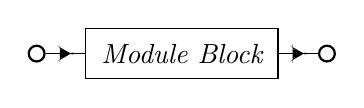
\begin{tikzpicture}
    \node[entry] (entry) {};
    \node[nterm] (mod) [right=of entry] {Module Block};
    \node[exit] (exit) [right=of mod] {};

    \draw[arr] (entry) -- (mod);
    \draw[arr] (mod) -- (exit);
  \end{tikzpicture}
\end{figure}

\subsection{Module Block}

One or more modules.

\begin{figure}[H]
  \centering
  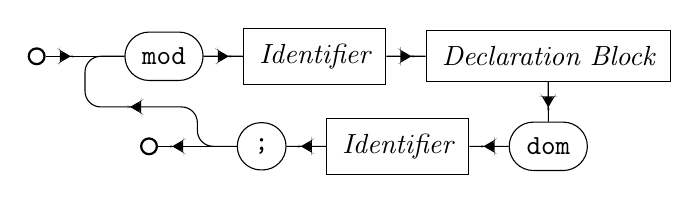
\begin{tikzpicture}
    \node[entry] (entry) {};
    \coordinate[right=of entry] (entry-mod);
    \node[term] (mod) [right=of entry-mod] {mod};
    \node[nterm] (name) [right=of mod] {Identifier};
    \node[nterm] (decl) [right=of name] {Declaration Block};
    \node[term] (dom) [below=of decl] {dom};
    \node[nterm] (exit name) [left=of dom] {Identifier};
    \node[term] (semi) [left=of exit name] {;};
    \coordinate[left=of semi] (semi-exit);
    \node[exit] (exit) [left=of semi-exit] {};

    \draw[arr] (entry) -- (entry-mod);
    \draw[narr] (entry-mod) -- (mod);

    \draw[arrs] (mod)
      -- (name)
      -- (decl)
      -- (dom)
      -- (exit name)
      -- (semi);

    \draw[narr] (semi) -- (semi-exit);
    \draw[arr] (semi-exit) -- (exit);

    \draw[arr] (semi)
      -- (semi-exit)
      -- ++(0, 0.5)
      -| (entry-mod)
      -- (mod);
  \end{tikzpicture}
\end{figure}

\subsection{Declaration Block}

A series of declarations

\begin{figure}[H]
  \centering
  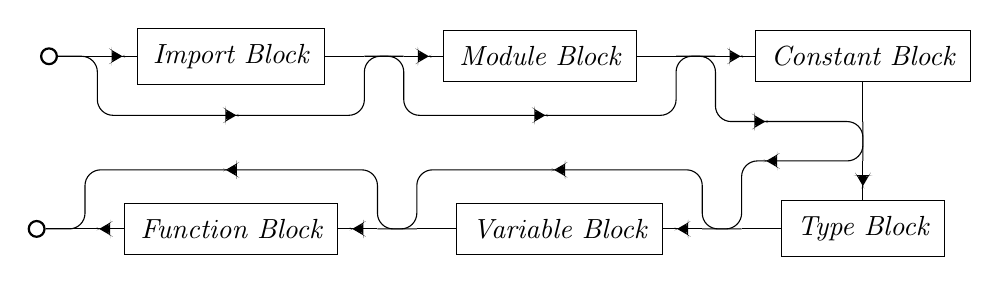
\begin{tikzpicture}
    \node[entry] (entry) {};
    \coordinate[right=of entry] (entry-imports);

    \node[nterm] (imports) [right=of entry-imports] {Import Block};
    \coordinate[right=of imports] (imports-mods 1);
    \coordinate[right=of imports-mods 1] (imports-mods 2);

    \node[nterm] (mods) [right=of imports-mods 2] {Module Block};
    \coordinate[right=of mods] (mods-consts 1);
    \coordinate[right=of mods-consts 1] (mods-consts 2);

    \node[nterm] (consts) [right=of mods-consts 2] {Constant Block};
    \coordinate[below=of consts] (consts-types 1);
    \coordinate[below=of consts-types 1] (consts-types 2);

    \node[nterm] (types) [below=of consts-types 2] {Type Block};
    \coordinate[left=of types] (types-vars 1);
    \coordinate[left=of types-vars 1] (types-vars 2);

    \node[nterm] (vars) [left=of types-vars 2] {Variable Block};
    \coordinate[left=of vars] (vars-funcs 1);
    \coordinate[left=of vars-funcs 1] (vars-funcs 2);

    \node[nterm] (funcs) [left=of vars-funcs 2] {Function Block};
    \coordinate[left=of funcs] (funcs-exit);

    \node[exit] (exit) [left=of funcs-exit] {};

    % main path
    \draw[narr] (entry) -- (entry-imports);
    \draw[arr] (entry-imports) -- (imports);
    
    \draw[narr] (imports) -- (imports-mods 1);
    \draw[arr] (imports-mods 2) -- (mods);

    \draw[narr] (mods) -- (mods-consts 1);
    \draw[arr] (mods-consts 2) -- (consts);

    \draw[narr] (consts) -- (consts-types 1);
    \draw[arr] (consts-types 2) -- (types);
      
    \draw[narr] (types) -- (types-vars 1);
    \draw[arr] (types-vars 2) -- (vars);

    \draw[narr] (vars) -- (vars-funcs 1);
    \draw[arr] (vars-funcs 2) -- (funcs);

    \draw[arr] (funcs) -- (funcs-exit);
    \draw[narr] (funcs-exit) -- (exit);
    
    % side path
    \draw[arr] (entry)
      -- (entry-imports)
      -- ++(0, -0.75)
      -| (imports-mods 1)
      -- (imports-mods 2);

    \draw[arr] (imports-mods 1)
      -- (imports-mods 2)
      -- ++(0, -0.75)
      -| (mods-consts 1)
      -- (mods-consts 2);

    \draw[arr] (mods-consts 1)
      -- (mods-consts 2)
      |- (consts-types 1)
      -- (consts-types 2);

    \draw[arr] (consts-types 1)
      -- (consts-types 2)
      -| (types-vars 1)
      -- (types-vars 2);

    \draw[arr] (types-vars 1)
      -- (types-vars 2)
      -- ++(0, 0.75)
      -| (vars-funcs 1)
      -- (vars-funcs 2);

    \draw[arr] (vars-funcs 1)
      -- (vars-funcs 2)
      -- ++(0, 0.75)
      -| (funcs-exit)
      -- (exit);
  \end{tikzpicture}
\end{figure}

\subsection{Import Block}

One or more import declarations.

\begin{figure}[H]
  \centering
  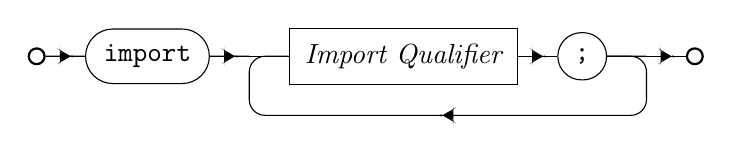
\begin{tikzpicture}
    \node[entry] (entry) {};
    \node[term] (import) [right=of entry] {import};
    \coordinate[right=of import] (import-qualifier);
    \node[nterm] (qualifier) [right=of import-qualifier] {Import Qualifier};
    \node[term] (semi) [right=of qualifier] {;};
    \coordinate[right=of semi] (semi-exit);
    \node[exit] (exit) [right=of semi-exit] {};

    \draw[arrs] (entry)
      -- (import)
      -- (import-qualifier);

    \draw[narr] (import-qualifier)
      -- (qualifier);

    \draw[arr] (qualifier) -- (semi);

    \draw[narr] (semi) -- (semi-exit);

    \draw[arr] (semi-exit) -- (exit);

    \draw[arr] (semi)
      -- (semi-exit)
      -- ++(0, -0.75)
      -| (import-qualifier)
      -- (qualifier);
  \end{tikzpicture}
\end{figure}

\subsubsection{Import Qualifier}

A qualifying series of identifiers for a module.

\begin{figure}[H]
  \centering
  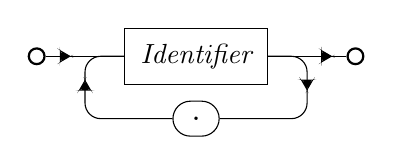
\begin{tikzpicture}
    \node[entry] (entry) {};
    \coordinate[right=of entry] (entry-name);
    \node[nterm] (name) [right=of entry-name] {Identifier};
    \coordinate[right=of name] (name-exit);
    \node[exit] (exit) [right=of name-exit] {};

    \node[term, node distance = 0.2cm] (dot) [below=of name] {.};

    \draw[arr] (entry) -- (entry-name);
    
    \draw[narr] (entry-name)
      -- (name)
      -- (name-exit);

    \draw[arr] (name-exit) -- (exit);

    \draw[narr, mid arrow = 0.35] (name)
      -- (name-exit)
      |- (dot);

    \draw[narr, mid arrow = 0.65] (dot)
      -| (entry-name)
      -- (name);
  \end{tikzpicture}
\end{figure}

\subsection{Constant Block}

One or more constant declarations.

\begin{figure}[H]
  \centering
  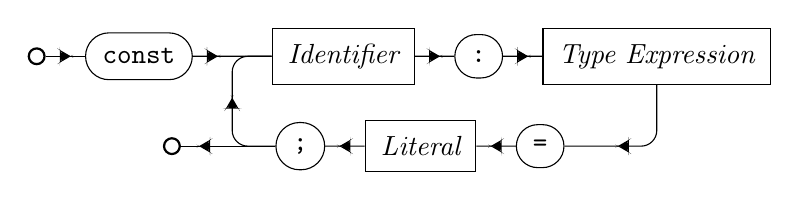
\begin{tikzpicture}
    \node[entry] (entry) {};
    \node[term] (const) [right=of entry] {const};
    \coordinate[right=of const] (const-name);
    \node[nterm] (name) [right=of const-name] {Identifier};
    \node[term] (colon) [right=of name] {:};
    \node[nterm] (type) [right=of colon] {Type Expression};
    \node[term] (eq) [below left=0.5cm and 0cm of type] {=};
    \node[nterm] (literal) [left=of eq] {Literal};
    \node[term] (semi) [left=of literal] {;};
    \node[exit] (exit) [left=1.2cm of semi] {};

    \draw[arrs] (entry) -- (const);
    \draw[narr, mid arrow = 0.25] (const) -- (name);
    \draw[arrs] (name)
      -- (colon)
      -- (type);

    \draw[narr, mid arrow = 0.6] (type) |- (eq);

    \draw[arrs] (eq)
      -- (literal)
      -- (semi);

    \draw[narr, mid arrow = 0.75] (semi) -- (exit);
    
    \draw[arr] (semi) -| (const-name) -- (name);

  \end{tikzpicture}
\end{figure}

\subsection{Variable Block}

One or more variable declarations.

\begin{figure}[H]
  \centering
  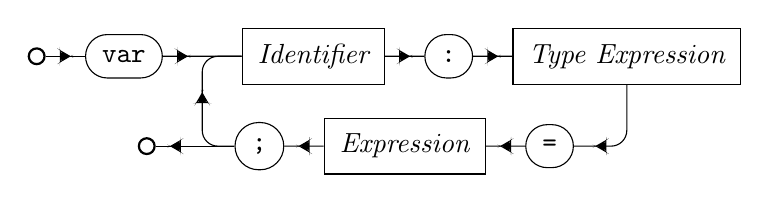
\begin{tikzpicture}
    \node[entry] (entry) {};
    \node[term] (var) [right=of entry] {var};
    \coordinate[right=of var] (var-name);
    \node[nterm] (name) [right=of var-name] {Identifier};
    \node[term] (colon) [right=of name] {:};
    \node[nterm] (type) [right=of colon] {Type Expression};
    \node[term] (eq) [below left=0.5cm and -0.5cm of type] {=};
    \node[nterm] (expr) [left=of eq] {Expression};
    \node[term] (semi) [left=of expr] {;};
    \node[exit] (exit) [left=1cm of semi] {};

    \draw[arrs] (entry) -- (var);
    \draw[narr, mid arrow = 0.25] (var) -- (name);
    \draw[arrs] (name)
      -- (colon)
      -- (type);

    \draw[narr, mid arrow = 0.75] (type) |- (eq);

    \draw[arrs] (eq)
      -- (expr)
      -- (semi);

    \draw[narr, mid arrow = 0.75] (semi) -- (exit);
    
    \draw[arr] (semi) -| (var-name) -- (name);

  \end{tikzpicture}
\end{figure}

\end{document}

